\chapter{Essentials}


\section{Cosmic radiation}
The cosmos is filled with particles of many kinds and sources.
Whereas the travel direction of charged particles is constantly bend by electromagnetic fields on their journey through space,
uncharged particles like gamma rays preserve their direction during their voyage.
This circumstances allow to identify their source.
Source specific characteristics can be found by determining the particle's properties.

\begin{figure}
    \centering
    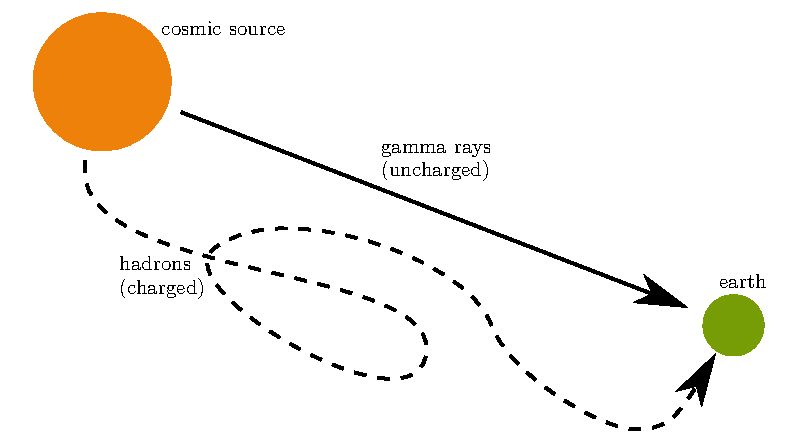
\includegraphics[scale=1]{Plots/Cosmic_Radiation.pdf}
    \caption{Uncharged particles propagate straight and charged particles propagate unpredictable through space.}
    \label{fig:cosmic_radiation}
\end{figure}

Gamma particles as well as hadrons can not cut through the earth's aerosphere and collide therefore with it.
Upon this collision the cosmic particle transfers some of it's energy the it's collision partner.
This causes an air shower by reason of the high energies in the \si{\tera\eV} range involved.
Since the speed of light in air is lower than in space some air shower particles can be faster than the light speed in air
without violating the cosmic speed of light.
In this case those particles emit a cone of Cherenkov radiation.
When a high energetic cosmic particle interacts with the aerosphere, a short flash of Cherenkov light can be detected at ground-level.

\begin{figure}
    \centering
    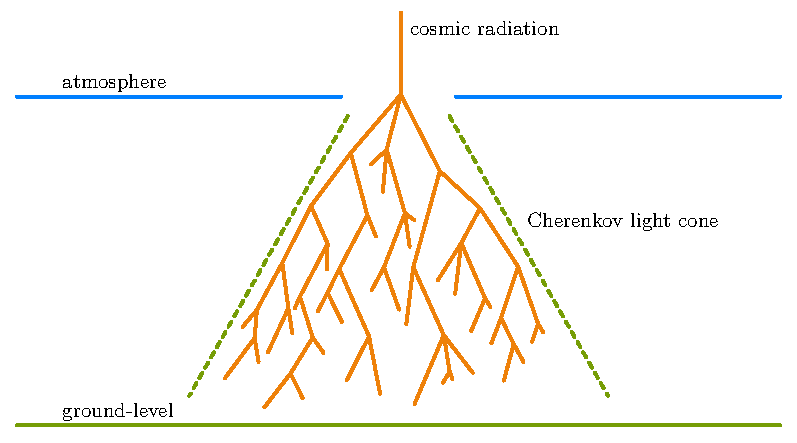
\includegraphics[scale=1]{Plots/Air_Shower.pdf}
    \caption{Cosmic particles cause Cherenkov light emitting air showers in the aerosphere by colliding with it.}
    \label{fig:air_shower}
\end{figure}


\section{FACT telescope}
Among other telescopes the First G-APD Cherenkov Telescope (FACT) on La Palma records these light flashes.
It uses Geiger-mode avalanche photodiods (G-APDs) as photo sensors for a test benchmark of this technology.
With its small mirror surface of \num{9.5}\,\si{\meter²} it operates since \num{2011}
and collects data of air showers caused by cosmic radiation in the TeV energy range.

The \num{1440} camera pixels form a hexagonal grid.
This hexagonal pixel structure represents a challenge for the further image processing
since software for image classification was developed for images with quadratic pixels.
Therefor the camera image has to be transformed by using the pixel IDs to map the hexagonal to a quadratic grid structure.
Skewing the image by translating it to a different coordinate system and padding it with empty pixels
enables further processing without developing special software.
One drawback of this procedure is the loss of some direct neighborhood information
(hexagonal: \num{6} neighbors, quadratic: \num{4} neighbors) of every pixel.

\begin{figure}
    \centering
    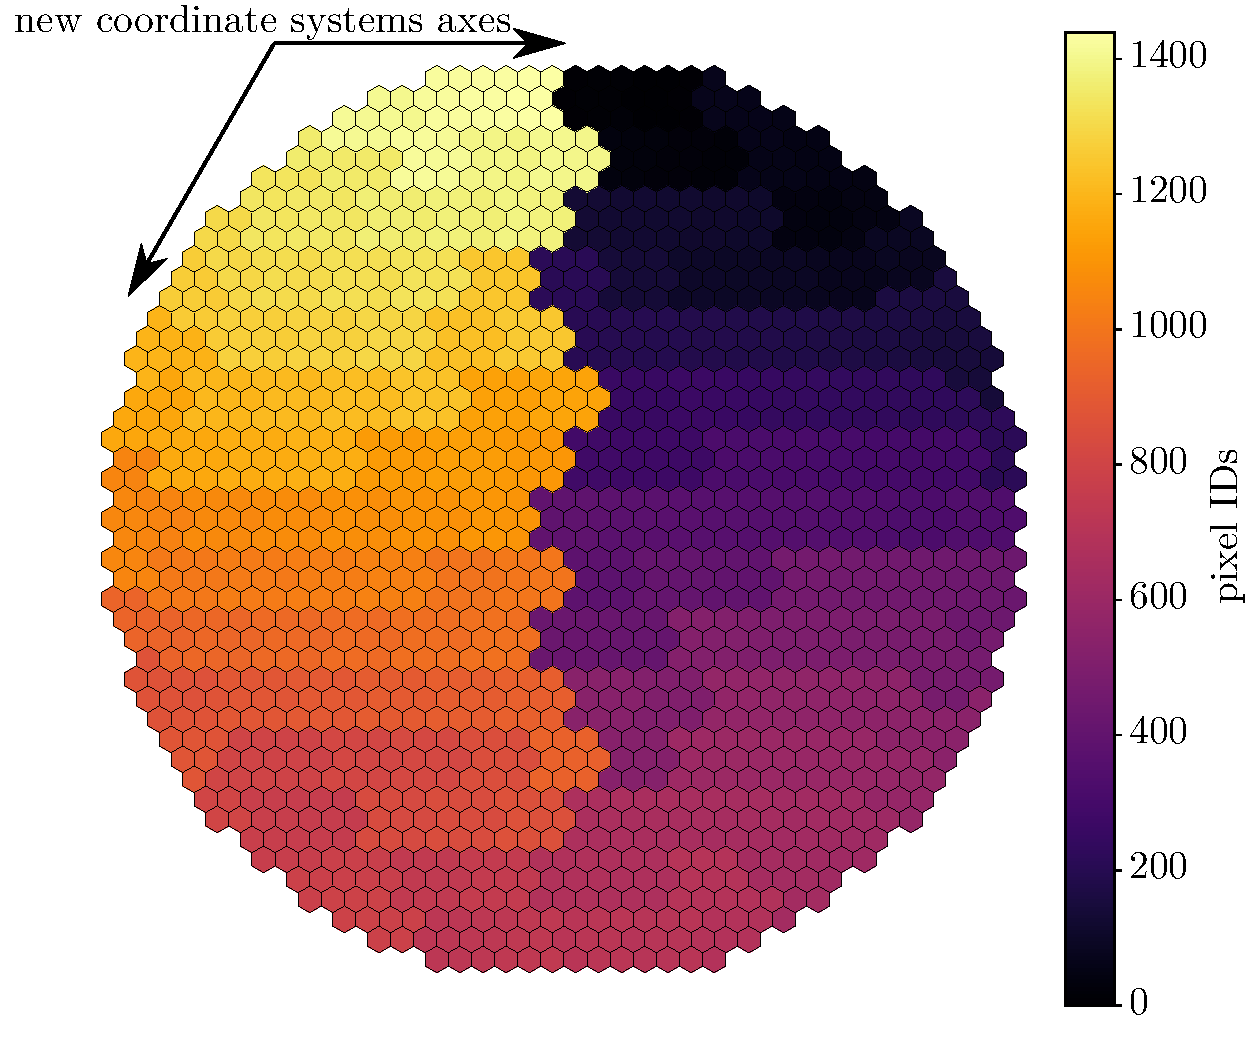
\includegraphics[width=100mm]{Plots/FACT_Image.pdf}
    \caption{Translating the FACT camera image to a new coordinate system by using the shown axes allows a transformation from a hexagonal to a quadratic grid structure.}
    \label{fig:fact_image}
\end{figure}

\begin{figure}
    \centering
    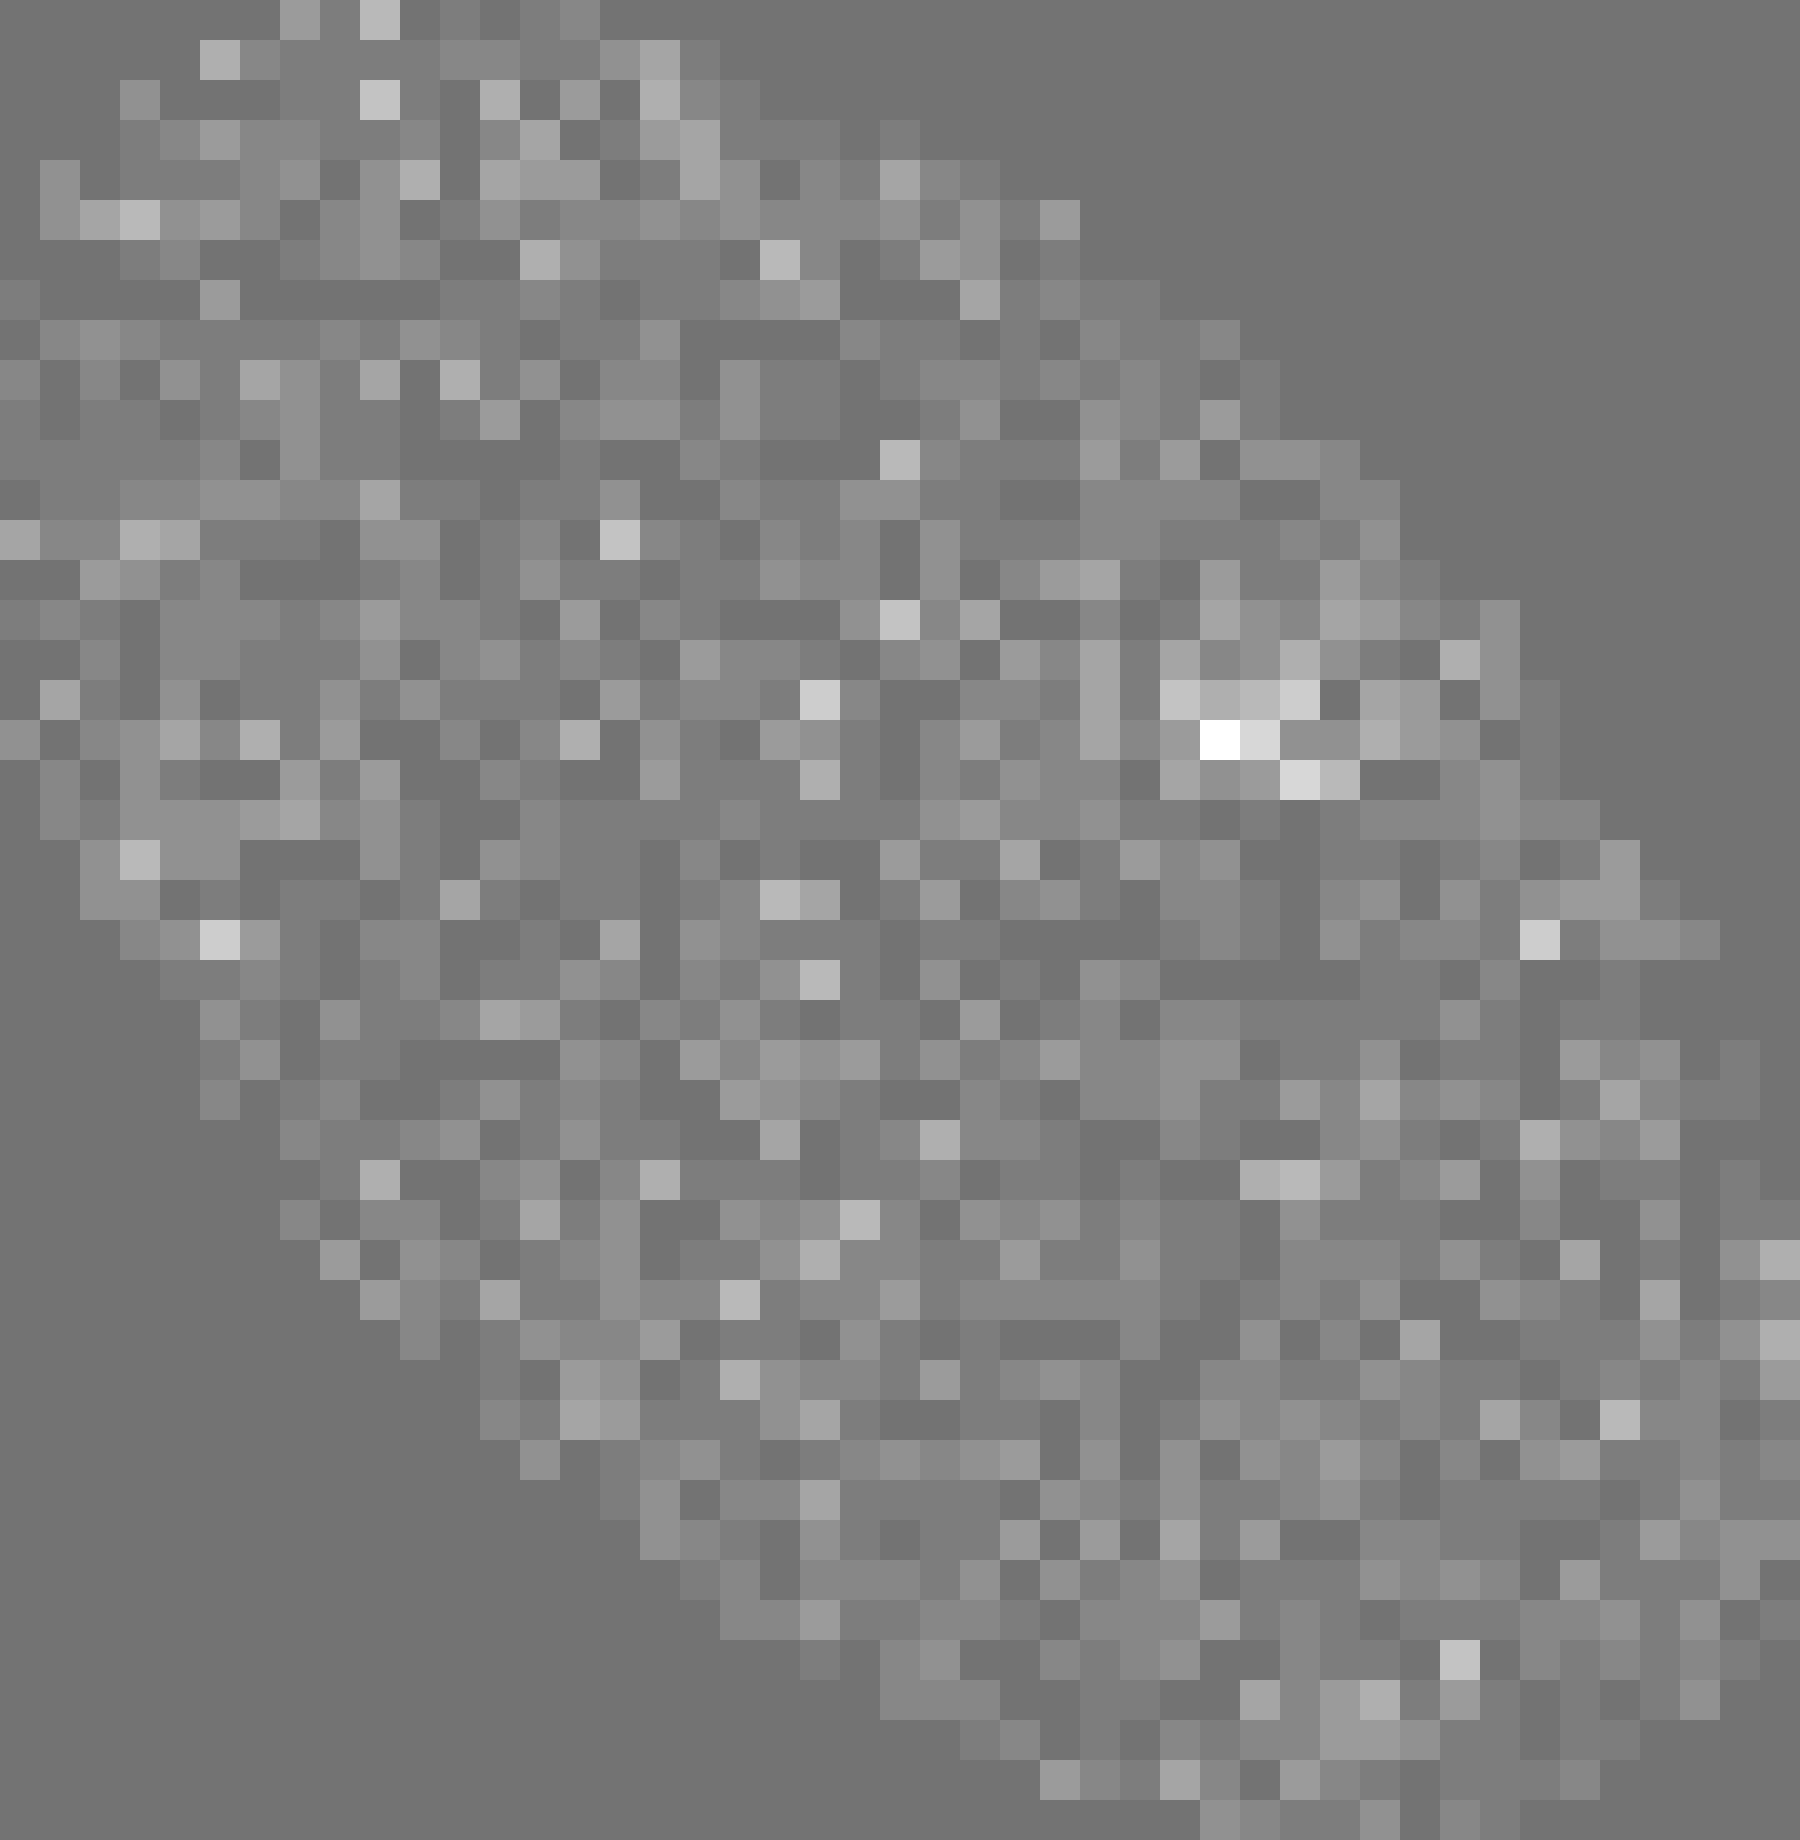
\includegraphics[width=60mm]{Plots/Preprocessed_Image.png}
    \caption{The transformed camera image will be padded with zeros and has a final size of \num{45} to \num{46} pixels.}
    \label{fig:preprocessed_image}
\end{figure}



\section{Convolutional Neural Networks}
In the recent years Deep Learning evolved at an incredible rate and generated impressive progress in image classification tasks.
Utilizing the progress this thesis tests the benefit of Convolutional Neural Networks (CNN) for classifying the skewed camera images
by their triggering cosmic particle.
To separate images caused by gammas or hadrons there are many possible architectures for the CNN.
Every architecture is composed of layers with different tasks.
The image will then be passed and transformed from layer to layer till it reaches the last one.

Convolution layers (depicted in the plots as 'c') act as feature generators.
Patterns in the image will be translation invariantly recognized therein.

Pooling layers reduce the feature space by selecting the most important ones.
They are following a convolution layer and will not be depicted in the plots.

Fully connected layers (depicted as 'f') complete the network in the final stages.
They combine the computed features and classify the image at the same time.

\begin{figure}
    \centering
    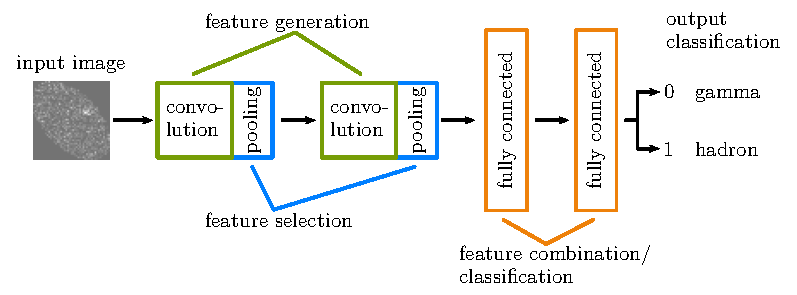
\includegraphics[scale=1]{Plots/CNN_Example.pdf}
    \caption{The input image will be transformed by every layer and passed onto the next one till it finally reaches the output layer classifying the image.}
    \label{fig:cnn_example}
\end{figure}

To minimize overfitting behavior and maximize generalization of the network different approaches can be used.
To attain evenly distributed pixel values normalization of every batch of images fed to the network is used (batch normalization).

At the cost of longer training times dropout layers ('d') can be inserted after any layer.
This will destroy some of the information flowing through the network
and force it to learn distributed representations of every feature making it more robust.

To enable long networks and faster training pretraining will be implemented.
After training small networks for a short time a new untrained layer will be attached.
This process will be iterated until the networks growth reached its final length.
While most of the layers only have to adapt slightly
the new layers can adjust their behavior according the pretrained network quickly.

For modeling the layers and the architectures Google's python library tensorflow has been used.
After creating the training programm's structure GPUs were used for training purposes
to utilize their parallel computing capabilities and cutting down the training time thereby.
Thats why the training times fluctuated roughly between \num{60}\,\si{\minute} and \num{120}\,\si{\minute} for a single network.
